\documentclass[conference]{IEEEtran}
\IEEEoverridecommandlockouts
% The preceding line is only needed to identify funding in the first footnote. If that is unneeded, please comment it out.
\usepackage{cite}
\usepackage{amsmath,amssymb,amsfonts}
\usepackage{algorithmic}
\usepackage{graphicx}
\usepackage{textcomp}
\usepackage{xcolor}
\usepackage{booktabs}
\usepackage{tabularx}
\usepackage{hyperref}
\usepackage{algorithm}  
%\usepackage{algorithmicx}  
\usepackage{algorithmic}
%\usepackage{algpseudocode}
 \usepackage{float}
\def\BibTeX{{\rm B\kern-.05em{\sc i\kern-.025em b}\kern-.08em
		T\kern-.1667em\lower.7ex\hbox{E}\kern-.125emX}}
\begin{document}
	
	\title{Investigation in extended kalman filter for indoor robot navigation\\
%		{\footnotesize \textsuperscript{*}Note: Sub-titles are not captured in Xplore and
%			should not be used}
%		\thanks{Identify applicable funding agency here. If none, delete this.}
	}
	
	\author{\IEEEauthorblockN{1\textsuperscript{st} Yihui Chen}
		\IEEEauthorblockA{\textit{National University of Singapore} \\
			e1010473@u.nus.edu}
	}
	
	\maketitle
	
	\begin{abstract}
		This document is a model and instructions for \LaTeX.
		This and the IEEEtran.cls file define the components of your paper [title, text, heads, etc.]. *CRITICAL: Do Not Use Symbols, Special Characters, Footnotes, 
		or Math in Paper Title or Abstract.
	\end{abstract}
	
	\begin{IEEEkeywords}
		component, formatting, style, styling, insert
	\end{IEEEkeywords}
	
	\section{Literature review}
	
	\section{Bayesian filter}
	
	\subsection{Bayes theorem in discrete and continuous cases}
	
	Bayes theorem describes the probability of an event based on prior knowledge. Suppose that random variable $X$ denote the event to be estimated while $Y$ represent the observation result, $x$ and $y$ are their specific values respectively. Consdier Bayes rule in discrete cases and get
	
	\begin{equation}
		P(X=x\mid Y=y)=\frac{P(Y=y\mid X=x)P(X=x)}{P(Y=y)}
		\label{eq1}
	\end{equation}
	
	where $P(Y=y\mid X=x)$ is likelyhood that often describes the measurement accuracy of sensor, and $P(X=x)$ denotes the prior probability based on current knowledge. Using the law of total probability, $P(Y=y)$ on the denominator can be expanded as $P(Y=y)=\sum_{i=1}^{n}P(Y=y \mid X=x_{i})P(X=x_{i})$, which shows that its value is not related to the value of $Y$ and thus it can be replaced by a constant $\eta $. Then Bayes theorem combines them and gives the posterior probability.
	
	Now consider the Bayes fomula for continuous random variables
	
	\begin{equation}
	P(X<x\mid Y=y)=\frac{P(Y=y\mid X<x)P(X<x)}{P(Y=y)}
	\label{eq2}
	\end{equation}
	
	Since the fomula can not be directly used, the right side is written as a sum of discrete probabilities and turned into a limit form. 
	
	\begin{equation}
	\begin{split}
	\begin{aligned}
	&RHS=\sum_{u=-\infty}^{x}\frac{P(Y=y\mid X=u)P(X=u)}{P(Y=y)}
	\\
	&=\lim_{\varepsilon \rightarrow 0}\sum_{u=-\infty}^{x}\frac{P(y<Y<y+\varepsilon \mid X=u)P(u<X<u+\varepsilon )}{P(y<Y<y+\varepsilon )}
	\nonumber
	\end{aligned}
	\end{split}
	\end{equation}
	
	Let $f(\cdot )$ denotes the probability density function and apply mean value theorem, we derive
	
	\begin{equation}
	\begin{split}
	\begin{aligned}
	RHS&=\lim_{\varepsilon_{1}, \varepsilon_{2}, \varepsilon_{3} \rightarrow 0}\sum_{u=-\infty}^{x} \frac{(f_{Y\mid X}(\xi _{1}\mid u)) (f_{X}(\xi _{2}))\cdot \varepsilon_{1} \varepsilon_{2}}{f_{Y}
		(\xi _{3})\cdot \varepsilon_{3}}\\
	&=\lim_{\varepsilon \rightarrow 0}\sum_{u=-\infty}^{x}\frac{f_{Y\mid X}(y\mid u)f_{X}(u)}{f_{Y}(y)}\cdot \varepsilon\\ 
	&=\int_{-\infty}^{x}\frac{f_{Y\mid X}(y\mid x)f_{X}(x)}{f_{Y}(y)}dx
	\nonumber
	\end{aligned}
	\end{split}
	\end{equation}
	
	where $\xi _{1}\in (y,y+\varepsilon_{1})$, $\xi _{2}\in (u,u+\varepsilon_{2})$ and $\xi _{3}\in (y,y+\varepsilon_{3})$. Also write the left side of Eq.~\ref{eq2} in a form of probability density function, i.e. $LHS=\int_{-\infty}^{x}f_{X\mid Y}(x\mid y)dx$, we finally get the Bayes formula for pdf in continuous cases.
	
	\begin{equation}
		f_{X\mid Y}(x\mid y)=\frac{f_{Y\mid X}(y\mid x)f_{X}(x)}{f_{Y}(y)}
		\label{eq3}
	\end{equation}
	
	Similarily, the denominator can be replace by a constant $\eta$, where $\eta=[\int_{-\infty}^{+\infty}f_{Y\mid X}(y\mid x)f_{X}(x)dx]^{-1}$. 
	
	\subsection{Bayesian filtering algorithm}
	
	Suppose we have established the prediction and observation equation as
	
	\begin{equation}
	\begin{split}
	\begin{aligned}
	X_{k}&=F(X_{k-1})+Q_{k}\\
	Y_{k}&=H(X_{k})+R_{k}
	\label{eq4}
	\end{aligned}
	\end{split}
	\end{equation}
	
	where $X_{k}$, $Y_{k}$, $Q_{k}$, $R_{k}$ are all random variables, and $X_{0}$, $Q_{k}$ and $R_{k}$ are mutually independent. In the prediction step, pdf of prior estimation $f_{k}^{-}(x)$ is firstly calculated.
	
	\begin{equation}
		f_{k}^{-}(x)=\frac{d}{dx}(P(X_{k}<x))=\frac{d}{dx}(\sum_{u=-\infty}^{x}P(X_{k}=u))
		\label{eq5}
	\end{equation}
	
	Expand $P(X_{k}=u)$ by total probability law and substitute the prediction function into it, we get
	
	\begin{equation}
	\begin{split}
	\begin{aligned}
	&P(X_{k}=u)=\sum_{v=-\infty}^{+\infty}P(X_{k}=u\mid X_{k-1}=v)P(X_{k-1}=v)\\
	&=\sum_{v=-\infty}^{+\infty}P(X_{k}-F(X_{k-1})=u-F(v)\mid X_{k-1}=v)P(X_{k-1}=v)\\
	&=\sum_{v=-\infty}^{+\infty}P(Q_{k}=u-F(v))P(X_{k-1}=v)
	\nonumber
	\end{aligned}
	\end{split}
	\end{equation}
	
	Repeat what we do on $RHS$ of Eq.~\ref{eq2}, it becomes
	
	\begin{equation}
	\begin{split}
	\begin{aligned}
	P(X_{k}=u)&=\lim_{\varepsilon \rightarrow 0 }\sum_{v=-\infty}^{+\infty}f_{Q_{k}}[u-F(v)]f_{k-1}(v)\cdot \varepsilon ^{2}\\
	&=\lim_{\varepsilon \rightarrow 0}\int_{-\infty}^{+\infty}f_{Q_{k}}[u-F(v)]f_{k-1}(v)dv \cdot \varepsilon
	\nonumber
	\end{aligned}
	\end{split}
	\end{equation}
	
	Substitute it into Eq.~\ref{eq5} and get the pdf of prior estimation
	
	\begin{equation}
	\begin{split}
	\begin{aligned}
	f_{k}^{-}(x)&=\frac{d}{dx}\begin{Bmatrix}
	{\sum_{-\infty}^{x}\lim_{\varepsilon \rightarrow 0}\int_{-\infty}^{+\infty}f_{Q_{k}}[u-F(v)]f_{k-1}(v)dv \cdot \varepsilon}
	\end{Bmatrix} \\
	&=\frac{d}{dx}\begin{Bmatrix}
	\int_{-\infty}^{x}\int_{-\infty}^{+\infty}f_{Q_{k}}[u-F(v)]f_{k-1}(v)dvdu)
	\end{Bmatrix}\\
	&=\int_{-\infty}^{+\infty}f_{Q_{k}}[x-F(v)]f_{k-1}(v)dv
	\label{eq6}
	\end{aligned}
	\end{split}
	\end{equation}
	
	After the observed value $Y_{k}=y_{k}$ is acquired by the sensor, the pdf of likelyhood is derived as
	
	\begin{equation}
	\begin{split}
	\begin{aligned}
	f_{Y_{k}\mid X_{k}}(y_{k}\mid x)&=\lim\limits_{\varepsilon \rightarrow 0}\frac{P(y_{k}<Y_{k}<y_{k}+\varepsilon\mid X_{k}=x)}{\varepsilon}\\
	&=\lim_{\varepsilon \rightarrow 0}\frac{P(y_{k}-H(x)<R_{k}<y_{k}-H(x)+\varepsilon)}{\varepsilon}\\
	&=f_{R_{k}}[y_{k}-H(x)]
	\label{eq7}
	\end{aligned}
	\end{split}
	\end{equation}
	
	Substitute Eq.~\ref{eq6} and Eq.~\ref{eq7} into Eq.~\ref{eq3}, we get the pdf of posterior estimation:
	
	\begin{equation}
		f_{k}^{+}(x)=\eta_{k} \cdot f_{R_{k}}[y_{k}-H(x)]\cdot f_{k}^{-}(x)
		\label{eq8}
	\end{equation}
	
	where $\eta_{k} = (\int_{-\infty}^{+\infty}f_{R_{k}}[y_{k}-H(x)]\cdot f_{k}^{-}(x)dx)^{-1}$. With the prediction and update steps, the current state of robot can be estimated realtime by Bayes formula. The algorithm flow is given below.

	
	\begin{algorithm}
		\caption{Bayesian filter}
		
		\begin{algorithmic}  
			\STATE INITIALIZE $f_{0}^{+}(x), Q, R$
			\FOR {i=1,...,r}
			\STATE Predict Step
			$f_{i}^{-}(x)=\int_{-\infty}^{+\infty}f_{Q_{i}}[x-F(v)]f_{i-1}^{+}(v)dv$
			\STATE Update Step
			$f_{i}^{+}(x)=\eta_{i}\cdot f_{R_{i}}[y_{i}-H(x)]f_{i}^{-}(x)$
			\STATE Estimate State $\hat{x}_{i}^{+}=\int_{-\infty}^{+\infty}xf_{i}^{+}(x)dx$
			\ENDFOR
		\end{algorithmic}
	\end{algorithm}
	
	\section{Kalman filter}
	
	\subsection{Kalman filter}
	
	Bayes filter estimates unknown probability density function recursively using a mathematical process model and external measurements, laying the foundation for realtime state estimation. However, it is usually hard to get analytical solutions when calculating improper integrals in the algorithm steps. Therefore, Kalman filter made some assumptions to simplify the process. Consider the prediction and observation equations in Eq.~\ref{eq4}, suppose that both $F(\cdot)$ and $H(\cdot)$ are linear functions, and $Q_{k}$, $R_{k}$ follow the normal distribution, i.e.
	
	\begin{equation}
	\begin{split}
	\begin{aligned}
	X_{k}&=FX_{k-1}+Q_{k}\\
	Y_{k}&=HX_{k}+R_{k}\\
	Q_{k}\sim N&(0,Q), R_{k}\sim N(0,R)
	\label{eq9}
	\end{aligned}
	\end{split}
	\end{equation}
	
	Then if the random variable at the last time also follows a normal distribution, i.e. $X_{k-1}^{+}\sim N(\mu _{k-1}^{+},\sigma  _{k-1}^{+})$, we can easily infer the pdf of prior probability is a normal distribution by convolution theorem.
	
	\begin{equation}
	\begin{split}
	\begin{aligned}
	FX_{k-1}^{+}&\sim N(F\mu _{k-1}^{+},F^{2}\sigma  _{k-1}^{+}), Q_{k}\sim N(0,Q)\\
	\Rightarrow X_{k}^{-}&\sim N(F\mu _{k-1}^{+},F^{2}\sigma  _{k-1}^{+}+Q)
	\label{eq10}
	\end{aligned}
	\end{split}
	\end{equation}
	
	Denote the mean and variance of $X_{k}^{-}$ as $\mu_{k}^{-}$ and $\sigma_{k}^{-}$, the pdf of posterior probability $f_{k}^{+}(x)$ and estimated state $\hat{x}_{k}^{+}$ can be derived following the update rule. Then the random variable $X_{k}^{+}$ at the current time also follows the normal distribution, i.e. $X_{k}^{+} \sim N(\mu_{k}^{+}, \sigma_{k}^{+})$, where $\hat{x}_{k}^{+}=\mu_{k}^{+}$ is the estimated state and they are given by
	
	\begin{equation}
	\begin{split}
	\begin{aligned}
	\mu_{k}^{+}&=\mu_{k}^{-}+K(y_{k}-H\mu_{k}^{-}) \\
	\sigma_{k}^{+}&=(1-KH)\sigma_{k}^{-}\\
	K&=\frac{H\sigma_{k}^{-}}{H^{2}\sigma_{k}^{-}+R}
	\label{eq11}
	\end{aligned}
	\end{split}
	\end{equation}
	
	Since the state variables are usually vectors, kalman filter algorithm can be generalized to a matrix form as below, where $\boldsymbol{F}$ and $\boldsymbol{H}$ are matrixes in prediction and observation equatons, and $\boldsymbol{\Sigma _{k}}$ is the covariance matrix.
	
	\begin{algorithm}
		\caption{Kalman filter}
		\begin{algorithmic}  
			\STATE Prediction equation $\boldsymbol{X_{k}}=\boldsymbol{F}\boldsymbol{X_{k-1}}+\boldsymbol{Q_{k}}$
			\STATE Observation equation $\boldsymbol{Y_{k}}=\boldsymbol{H}\boldsymbol{X_{k}}+\boldsymbol{R_{k}}$
			\STATE $\boldsymbol{Q_{k}}\sim N(\boldsymbol{0},\boldsymbol{Q})$, $\boldsymbol{R_{k}}\sim N(\boldsymbol{0},\boldsymbol{R})$, $\boldsymbol{X_{0}}\sim N(\boldsymbol{\mu_{0}^{+}}, \boldsymbol{\Sigma_{0}^{+}})$
			\STATE Initialize $ \boldsymbol{\mu_{0}^{+}}, \boldsymbol{\Sigma_{0}^{+}}, \boldsymbol{Q}, \boldsymbol{R}$
			\FOR {k=1,...,r}
			\STATE $\boldsymbol{\mu_{k}^{-}}=\boldsymbol{F}\boldsymbol{\mu_{k-1}^{+}}$ 
			\STATE $\boldsymbol{\Sigma_{k}^{-}}=\boldsymbol{F}\boldsymbol{\Sigma_{k-1}^{+}}\boldsymbol{F}^{T}+\boldsymbol{Q}$ \ \ \ \ \ \ \ \ \ \ \ \ \ \ \ \ \ \ \ \ \COMMENT{prediction end}
			\STATE $\boldsymbol{K}=\boldsymbol{\Sigma_{k}^{-}}\boldsymbol{H}^{T}(\boldsymbol{H}\boldsymbol{\Sigma_{k}^{-}}\boldsymbol{H}^{T}+\boldsymbol{R})^{-1}$ \ \ \ \ 	\COMMENT{the kalman gain}
			\STATE Obtain an observation value $\boldsymbol{y_{k}}$
			\STATE $\boldsymbol{\mu_{k}^{+}}=\boldsymbol{\mu_{k}^{-}}+\boldsymbol{K}(\boldsymbol{y_{k}}-\boldsymbol{H}\boldsymbol{\mu_{k}^{-}})^{-1}$
			\STATE $\boldsymbol{\Sigma_{k}^{+}}=(\boldsymbol{I}-\boldsymbol{KH})\boldsymbol{\Sigma_{k}^{-}}$ \ \ \ \ \ \ \ \ \ \ \ \ \ \ \ \ \ \ \ \ \ \ \ \COMMENT{update end}
			\STATE $\boldsymbol{\hat{x}_{k}^{+}}=\boldsymbol{\mu_{k}^{+}}$
			\ENDFOR
		\end{algorithmic}
	\end{algorithm}
	
	\subsection{Extended Kalman filter}
	
	Prediction and observation functions are usually nonlinear in real cases, but they are simply supposed to be linear in Kalman filter, which leads to bad performance. Extended Kalman filter improve it by linearizing them by Taylor series. We still suppose that $X_{k-1}^{+}\sim N(\mu_{k-1}^{+}, \sigma_{k-1}^{+})$, and expand $F(X_{k-1}^{+})$ by its first-order Taylor series about $\mu_{k-1}^{+}$ as
	
	\begin{equation}
	\begin{split}
	\begin{aligned}
	F(X_{k-1}^{+})&\approx F(\mu_{k-1}^{+})+{F}'(\mu_{k-1}^{+})(X_{k-1}^{+}-\mu_{k-1}^{+})\\
	&\approx AX_{k-1}^{+}+B
	\label{eq12}
	\end{aligned}
	\end{split}
	\end{equation}
	
	where $A={F}'(\mu_{k-1}^{+})$ and $B=F(\mu_{k-1}^{+})-{F}'(\mu_{k-1}^{+})\mu_{k-1}^{+}$. Similarly, we follow the prediction step in Bayes filter algorithm and find $X_{k}^{-}$ also follows the normal distribution, i.e. $X_{k}^{-} \sim N(A\mu_{k-1}^{+}+B, A^{2}\sigma_{k-1}^{+}+Q)$. Substitute $A$ and $B$ into it and it becomes
	
	\begin{equation}
		X_{k}^{-} \sim N(F(\mu_{k-1}^{+}), A^{2}\sigma_{k-1}^{+}+Q)
		\label{eq13}
	\end{equation}
	
	Denote the mean and variance in Eq.~\ref{eq13} are $\mu_{k}^{-}$ and $\sigma_{k}^{-}$ respectively, we calculate the pdf of posterior probability $f_{k}^{+}(x)$ by the update step in Bayes filter. Similarily, we expand the nonlinear observation function $H(X_{k})$ by Taylor series about $\mu_{k}^{-}$ as
	
	\begin{equation}
	\begin{split}
	\begin{aligned}
	H(X_{k})&\approx H(\mu_{k}^{-})+{H}'(\mu_{k}^{-})(X_{k}-\mu_{k}^{-})\\
	&\approx CX_{k}+D
	\label{eq14}
	\end{aligned}
	\end{split}
	\end{equation}
	
	where $C={H}'(\mu_{k}^{-})$ and $D=H(\mu_{k}^{-})-{H}'(\mu_{k}^{-})\mu_{k}^{-}$. Following the update step we find the pdf of posterior probability is also in shape of normal distribution. Therefore, the random variable after update follows 
	
	\begin{equation}
	\begin{split}
	\begin{aligned}
	X_{k}^{+} &\sim N(\frac{R\mu_{k}^{-}+C\sigma_{k}^{-}(y_{k}-D)}{R+C^{2}\sigma_{k}^{-}}, (1-\frac{C^{2}\sigma_{k}^{-}}{R+C^{2}\sigma_{k}^{-}})\sigma_{k}^{-})\\
	&\sim N(\mu_{k}^{-}+K(y_{k}-H(\mu_{k}^{-})), (1-KC)\sigma_{k}^{-})
	\label{eq15}
	\end{aligned}
	\end{split}
	\end{equation}
	
	where $K=\frac{C\sigma_{k}^{-}}{R+C^{2}\sigma_{k}^{-}}$. Then we get our estimated state $x_{k}^{+}=\mu_{k}^{+}$. We can also generate the extended Kalman filter into matrix case. Different from the scalar case, here $\boldsymbol{Q}$, $\boldsymbol{R}$, $\boldsymbol{\Sigma_{k}}$ are all covariance matrixes, and $\boldsymbol{A}_{n\times n}$, $\boldsymbol{C}_{m\times n}$ ($m$ observers and $n$ state variables) need to be calculated in each loop:
	
	\begin{equation}
	\boldsymbol{A}=\begin{pmatrix}
	\frac{\partial F_{1}}{\partial X_{k-1}^{1}} &\frac{\partial F_{1}}{\partial X_{k-1}^{2}}  &\cdots   &\frac{\partial F_{1}}{\partial X_{k-1}^{n}} \\ 
	\frac{\partial F_{2}}{\partial X_{k-1}^{1}} &\frac{\partial F_{2}}{\partial X_{k-1}^{2}}  &\cdots   &\frac{\partial F_{2}}{\partial X_{k-1}^{n}} \\ 
	\vdots  &\vdots   &\ddots   &\vdots  \\ 
	\frac{\partial F_{n}}{\partial X_{k-1}^{1}} &\frac{\partial F_{n}}{\partial X_{k-1}^{2}}  &\cdots   & \frac{\partial F_{n}}{\partial X_{k-1}^{n}}
	\end{pmatrix}_{\mid X_{k-1}=\hat{x}_{k-1}^{+}=\mu_{k-1}^{+}}\\
	\label{eq16}
	\end{equation}
	
	\begin{equation}
	\boldsymbol{C}=\begin{pmatrix}
	\frac{\partial H_{1}}{\partial X_{k}^{1}} &\frac{\partial H_{1}}{\partial X_{k}^{2}}  &\cdots   &\frac{\partial H_{1}}{\partial X_{k}^{2}} \\ 
	\vdots  &\vdots   &\ddots   &\vdots  \\ 
	\frac{\partial H_{m}}{\partial X_{k}^{1}} &\frac{\partial H_{m}}{\partial X_{k}^{2}}  &\cdots   &\frac{\partial H_{m}}{\partial X_{k}^{n}} 
	\end{pmatrix}_{\mid X_{k}=\hat{x}_{k}^{-}=\mu_{k}^{-}} 
	\label{eq17}
	\end{equation}
	
	
	
	The full flow of EKF algorithm is shown below.
	
	\begin{algorithm}
		\caption{Extended Kalman filter}
		\begin{algorithmic}  
			\STATE Prediction equation $\boldsymbol{X_{k}}=\boldsymbol{F}(\boldsymbol{X_{k-1}})+\boldsymbol{Q_{k}}$
			\STATE Observation equation $\boldsymbol{Y_{k}}=\boldsymbol{H}(\boldsymbol{X_{k}})+\boldsymbol{R_{k}}$
			\STATE $\boldsymbol{Q_{k}}\sim N(\boldsymbol{0},\boldsymbol{Q})$, $\boldsymbol{R_{k}}\sim N(\boldsymbol{0},\boldsymbol{R})$, $\boldsymbol{X_{0}}\sim N(\boldsymbol{\mu_{0}^{+}}, \boldsymbol{\Sigma_{0}^{+}})$
			\STATE Initialize $ \boldsymbol{\mu_{0}^{+}}, \boldsymbol{\Sigma_{0}^{+}}, \boldsymbol{Q}, \boldsymbol{R}$
			\FOR {k=1,...,r}
			\STATE Calculate $\boldsymbol{A}$ using Eq.~\ref{eq16}
			\STATE $\boldsymbol{\mu_{k}^{-}}=\boldsymbol{F}(\boldsymbol{\mu_{k-1}^{+}})$ 
			\STATE $\boldsymbol{\Sigma_{k}^{-}}=\boldsymbol{A}\boldsymbol{\Sigma_{k-1}^{+}}\boldsymbol{A}^{T}+\boldsymbol{Q}$ \ \ \ \ \ \ \ \ \ \ \ \ \ \ \ \ \ \ \ \ \COMMENT{prediction end}
			\STATE Calculate $\boldsymbol{C}$ using Eq.~\ref{eq17}
			\STATE $\boldsymbol{K}=\boldsymbol{\Sigma_{k}^{-}}\boldsymbol{C}^{T}(\boldsymbol{C}\boldsymbol{\Sigma_{k}^{-}}\boldsymbol{C}^{T}+\boldsymbol{R})^{-1}$ \ \ \ \ 	\COMMENT{the kalman gain}
			\STATE Obtain an observation value $\boldsymbol{y_{k}}$
			\STATE $\boldsymbol{\mu_{k}^{+}}=\boldsymbol{\mu_{k}^{-}}+\boldsymbol{K}[\boldsymbol{y_{k}}-\boldsymbol{H}(\boldsymbol{\mu_{k}^{-}})]^{-1}$
			\STATE $\boldsymbol{\Sigma_{k}^{+}}=(\boldsymbol{I}-\boldsymbol{KC})\boldsymbol{\Sigma_{k}^{-}}$ \ \ \ \ \ \ \ \ \ \ \ \ \ \ \ \ \ \ \ \ \ \ \ \COMMENT{update end}
			\STATE $\boldsymbol{\hat{x}_{k}^{+}}=\boldsymbol{\mu_{k}^{+}}$
			\ENDFOR
		\end{algorithmic}
	\end{algorithm}
	
	\subsection{Test results}
	
	To test the performance of these filters, we create a signal $x_{1}(t)=t^{2}$ and suppose the sensor noise follows the gaussian distribution, i.e. $\omega_{1} \sim N(0,0.1)$. First we use Kalman filter and establish prediction and observation equations. Since $X_{k}$ can be expanded about $X_{k-1}$ as $X_{k}=X_{k-1}+{X_{k-1}}'dt+\frac{1}{2}{X_{k-1}}''(dt)^{2}$, we choose $\begin{pmatrix}
	X_{k-1} &{X_{k-1}}'  &{X_{k-1}}'' 
	\end{pmatrix}^{T}$ and the two equations becomes
	
	\begin{equation}
		\begin{pmatrix}
		X_{k}\\ 
		{X_{k}}'\\ 
		{X_{k}}''
		\end{pmatrix}=\begin{pmatrix}
		1 &dt  &\frac{1}{2}(dt)^{2} \\ 
		0 &1  &dt \\ 
		0 &0  &1 
		\end{pmatrix}\begin{pmatrix}
		X_{k-1}\\ 
		{X_{k-1}}'\\ 
		{X_{k-1}}''
		\end{pmatrix}+Q_{k}
		\label{eq18}
	\end{equation}
	
	\begin{equation}
	Y_{k}=\begin{pmatrix}
	1 &0  &0 
	\end{pmatrix}\begin{pmatrix}
	X_{k}\\ 
	{X_{k}}'\\ 
	{X_{k}}''
	\end{pmatrix}+R_{k}
	\label{eq19}
	\end{equation}
	
	where $Q_{k}\sim N(0,Q)$, $R_{k}\sim N(0,R)$. The prediction for the higher derivative is considered more accurate and sensor noise is a little bit large, so here let $Q=diag\begin{Bmatrix}
	1 &0.01  &0.0001 
	\end{Bmatrix}$ and $R=20$. Also, $\boldsymbol{\mu_{0}^{+}}$ and $\boldsymbol{\Sigma_{0}^{+}}$ are initialized as $\begin{pmatrix}
	0.01 &0  &0 
	\end{pmatrix}^{T}$ and $diag\begin{Bmatrix}
	0.01 &0.01  &0.0001 
	\end{Bmatrix}$ respectively. As shown in Fig.~\ref{fig1}, Kalman filter cut down the error between observation and real signals. 
	
	\begin{figure}[htbp]
		\centering
		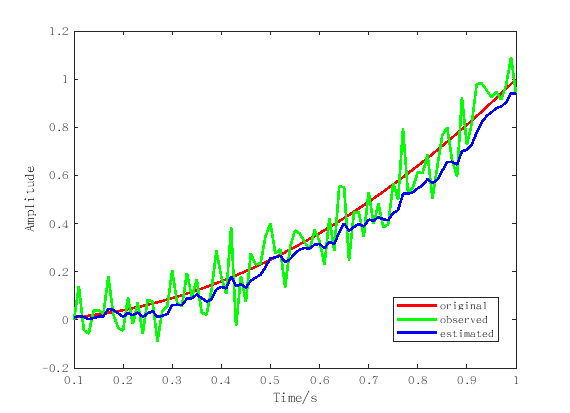
\includegraphics[width=8cm]{fig1.png}
		\caption{Estimation for $x_{1}(t)=t^{2}$ using Kalman filter with one sensor}
		\label{fig1}
	\end{figure}

	Now we add another sensor with higher measurement accuracy and modify the observation equation (Eq.~\ref{eq20}), where we tend to trust more on the second sensor and let $R=diag\begin{Bmatrix}
	3 &5
	\end{Bmatrix}$. The filtering result after sensor fusion is illustrated in Fig.~\ref{fig2}, where the estimation error is further reduced.
	
	\begin{equation}
	\begin{pmatrix}
	Y_{k_{1}}\\ 
	Y_{k_{2}}
	\end{pmatrix}=\begin{pmatrix}
	1 &0  &0 \\ 
	1 &0  & 0
	\end{pmatrix}\begin{pmatrix}
	X_{k}\\ 
	{X_{k}}'\\ 
	{X_{k}}''
	\end{pmatrix}+R_{k}
	\label{eq20}
	\end{equation}
	
	
	\begin{figure}[htbp]
		\centering
		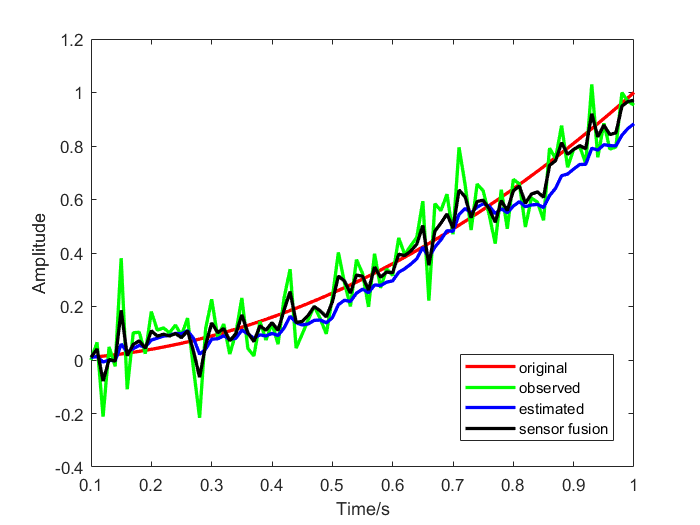
\includegraphics[width=8cm]{fig2.png}
		\caption{Estimation for $x_{1}(t)=t^{2}$ using Kalman filter after sensor fusion}
		\label{fig2}
	\end{figure}

	Then we choose another signal with stronger nonlinearity. The real signal $x_{2}(t)$ follows that  $x_{2}(t+1)=sin(3x_{2}(t))$ and $x_{2}(0)=0.1$. 
	
	
	\begin{figure}[htbp]
		\centering
		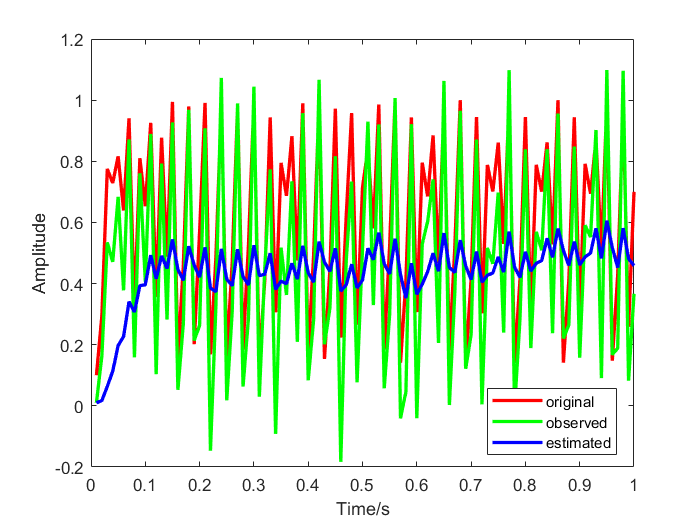
\includegraphics[width=8cm]{fig3.png}
		\caption{Estimation for $x_{2}(t)$ using Kalman filter}
		\label{fig3}
	\end{figure}
	
	\begin{figure}[htbp]
		\centering
		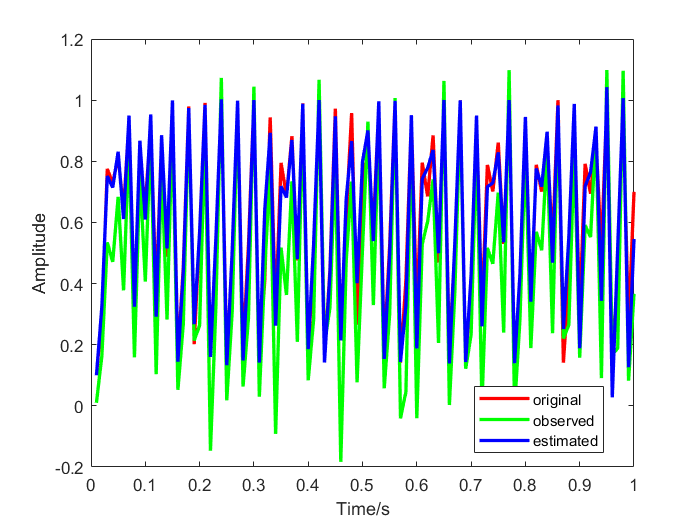
\includegraphics[width=8cm]{fig4.png}
		\caption{Estimation for $x_{2}(t)$ using extended Kalman filter}
		\label{fig4}
	\end{figure}
	
	\newpage
	
	\newpage
	
	
	
%	\subsection{Units}
%	\begin{itemize}
%		\item Use either SI (MKS) or CGS as primary units. (SI units are encouraged.) English units may be used as secondary units (in parentheses). An exception would be the use of English units as identifiers in trade, such as ``3.5-inch disk drive''.
%	\end{itemize}
	
%	\subsection{Equations}
%
%	\begin{equation}
%		a+b=\gamma\label{eq}
%	\end{equation}
%	 Use ``\eqref{eq}'', not ``Eq.~\eqref{eq}'' or ``equation \eqref{eq}'', except at 
%	the beginning of a sentence: ``Equation \eqref{eq} is . . .''
%	
%	\subsection{\LaTeX-Specific Advice}
%	
%	Please use ``soft'' (e.g., \verb|\eqref{Eq}|) cross references instead
%	of ``hard'' references (e.g., \verb|(1)|). That will make it possible
%	to combine sections, add equations, or change the order of figures or
%	citations without having to go through the file line by line.
%	
%	Please don't use the \verb|{eqnarray}| equation environment. Use
%	\verb|{align}| or \verb|{IEEEeqnarray}| instead. The \verb|{eqnarray}|
%	environment leaves unsightly spaces around relation symbols.
%	
%	
%	\subsection{Some Common Mistakes}\label{SCM}
%	\begin{itemize}
%		\item The word ``data'' is plural, not singular.
%	\end{itemize}
%	An excellent style manual for science writers is \cite{b7}.
%	
%	\subsection{Authors and Affiliations}
%	\textbf{The class file is designed for, but not limited to, six authors.} A 
%	minimum of one author is required for all conference articles. Author names 
%	should be listed starting from left to right and then moving down to the 
%	next line. This is the author sequence that will be used in future citations 
%	and by indexing services. Names should not be listed in columns nor group by 
%	affiliation. Please keep your affiliations as succinct as possible (for 
%	example, do not differentiate among departments of the same organization).
%	
%	\subsection{Identify the Headings}
%	Headings, or heads, are organizational devices that guide the reader through 
%	your paper. There are two types: component heads and text heads.
%	
%	\subsection{Figures and Tables}
%	\paragraph{Positioning Figures and Tables} Place figures and tables at the top and 
%	bottom of columns. Avoid placing them in the middle of columns. Large 
%	figures and tables may span across both columns. Figure captions should be 
%	below the figures; table heads should appear above the tables. Insert 
%	figures and tables after they are cited in the text. Use the abbreviation 
%	``Fig.~\ref{fig}'', even at the beginning of a sentence.
%	
%	\begin{table}[htbp]
%		\caption{Table Type Styles}
%		\begin{center}
%			\begin{tabular}{|c|c|c|c|}
%				\hline
%				\textbf{Table}&\multicolumn{3}{|c|}{\textbf{Table Column Head}} \\
%				\cline{2-4} 
%				\textbf{Head} & \textbf{\textit{Table column subhead}}& \textbf{\textit{Subhead}}& \textbf{\textit{Subhead}} \\
%				\hline
%				copy& More table copy$^{\mathrm{a}}$& &  \\
%				\hline
%				\multicolumn{4}{l}{$^{\mathrm{a}}$Sample of a Table footnote.}
%			\end{tabular}
%			\label{tab2}
%		\end{center}
%	\end{table}
%	
%	
	\section*{Acknowledgment}
	
	The preferred spelling of the word ``acknowledgment'' in America is without 
	an ``e'' after the ``g''. Avoid the stilted expression ``one of us (R. B. 
	G.) thanks $\ldots$''. Instead, try ``R. B. G. thanks$\ldots$''. Put sponsor 
	acknowledgments in the unnumbered footnote on the first page.
	
%	\section*{References}
	
%	Please number citations consecutively within brackets \cite{b1}. The 
%	sentence punctuation follows the bracket \cite{b2}. Refer simply to the reference 
%	number, as in \cite{b3}---do not use ``Ref. \cite{b3}'' or ``reference \cite{b3}'' except at 
%	the beginning of a sentence: ``Reference \cite{b3} was the first $\ldots$''
%	
%	Number footnotes separately in superscripts. Place the actual footnote at 
%	the bottom of the column in which it was cited. Do not put footnotes in the 
%	abstract or reference list. Use letters for table footnotes.
%	
%	Unless there are six authors or more give all authors' names; do not use 
%	``et al.''. Papers that have not been published, even if they have been 
%	submitted for publication, should be cited as ``unpublished'' \cite{b4}. Papers 
%	that have been accepted for publication should be cited as ``in press'' \cite{b5}. 
%	Capitalize only the first word in a paper title, except for proper nouns and 
%	element symbols.
%	
%	For papers published in translation journals, please give the English 
%	citation first, followed by the original foreign-language citation \cite{b6}.
	
%	\begin{thebibliography}{00}
%		\bibitem{b1} G. Eason, B. Noble, and I. N. Sneddon, ``On certain integrals of Lipschitz-Hankel type involving products of Bessel functions,'' Phil. Trans. Roy. Soc. London, vol. A247, pp. 529--551, April 1955.
%		\bibitem{b2} J. Clerk Maxwell, A Treatise on Electricity and Magnetism, 3rd ed., vol. 2. Oxford: Clarendon, 1892, pp.68--73.
%		\bibitem{b3} I. S. Jacobs and C. P. Bean, ``Fine particles, thin films and exchange anisotropy,'' in Magnetism, vol. III, G. T. Rado and H. Suhl, Eds. New York: Academic, 1963, pp. 271--350.
%		\bibitem{b4} K. Elissa, ``Title of paper if known,'' unpublished.
%		\bibitem{b5} R. Nicole, ``Title of paper with only first word capitalized,'' J. Name Stand. Abbrev., in press.
%		\bibitem{b6} Y. Yorozu, M. Hirano, K. Oka, and Y. Tagawa, ``Electron spectroscopy studies on magneto-optical media and plastic substrate interface,'' IEEE Transl. J. Magn. Japan, vol. 2, pp. 740--741, August 1987 [Digests 9th Annual Conf. Magnetics Japan, p. 301, 1982].
%		\bibitem{b7} M. Young, The Technical Writer's Handbook. Mill Valley, CA: University Science, 1989.
%	\end{thebibliography}

%	\bibliographystyle{IEEEtran}
%	
%	\bibliography{ref_5701}{}	
	
	
%	\vspace{12pt}
%	\color{red}
%	IEEE conference templates contain guidance text for composing and formatting conference papers. Please ensure that all template text is removed from your conference paper prior to submission to the conference. Failure to remove the template text from your paper may result in your paper not being published.
	
\end{document}
